\PassOptionsToPackage{dvipsnames}{xcolor}
\documentclass[14pt]{beamer}

\usepackage{biblatex}
\addbibresource{citations.bib}

\usepackage{amsmath}
\usepackage{mathtools}
\usepackage{emoji}
\usepackage{xfrac}
\usepackage{cancel}
\usepackage{csquotes}

\usepackage[]{xcolor}
\def\MyGreen{ForestGreen}
\def\MyRed{Red}
\def\MyOrange{BurntOrange}
\def\MyBlue{NavyBlue}
\definecolor{SuperLightGray}{rgb}{0.9,0.9,0.9}

\usepackage{calc}

% This lets us \includestandalone tikz pictures in standalone documents.
\usepackage{tikz}
\usetikzlibrary{tikzmark}
\usetikzlibrary{decorations.pathreplacing,calligraphy,backgrounds}
\usetikzlibrary{calc}
\usepackage[mode=buildnew]{standalone}
\usepackage{xifthen}

\makeatother
\renewcommand{\thefootnote}{
    \ifcase\value{footnote}
        \or*
        \or**
        \or***
        \or****
    \fi}
\makeatletter

\usefonttheme{serif}
\setbeamertemplate{navigation symbols}{}%remove navigation symbols

\setbeamerfont{title}{shape=\sc}
\setbeamerfont{frametitle}{shape=\sc}

\setbeamercolor{title}{fg=black}
\setbeamercolor{frametitle}{fg=black}

\setbeamercolor{enumerate item}{fg=gray}
\setbeamerfont{enumerate item}{shape=\bf}

\newcommand{\Seq}[1]{\left\{ {#1} \right\}}
\newcommand{\Exp}[1]{e^{#1}}

\title{A parallel SPH implementation on multi-core
        CPUs\\[.1em]
    {\scriptsize (2010)}
}
\author{
    \small{Ihmsen, M., Nadir, A., Becker, N., Teschner, M.}\\[2em]
    \scriptsize{\color{gray}presented by Steffen Haug}
}
\date{}

\begin{document}

%%
\begin{frame}
\titlepage
\end{frame}


%%
\begin{frame}
\centering
{\scriptsize\textsc{
A parallel \underline{SPH} implementation
on \underline{multi-core CPUs}
}}
\\[2em]

\onslide<2>{
    Applies to particle simulations in general!\\
    {\scriptsize (And raytracing, rigid body collision, ...)}
}
\end{frame}

%%
\begin{frame}
\centering
\textsc{Smoothed-particle Hydrodynamics}\\{\scriptsize
(Briefly)}
\end{frame}

%%
\begin{frame}
\centering
{
\begin{minipage}[c][.7\textheight][t]{.9\textwidth}
\centering
\textsc{\scriptsize Smoothed-particle Hydrodynamics}\\[1em]

\begin{equation*}
    A(x) = \int_\Omega A(V)  \delta(x - V) dV
\end{equation*}

\vfill
{\scriptsize Start with the convolution definition of $\delta$.}
\end{minipage}
}
\end{frame}

%%
\begin{frame}
\centering
{
\begin{minipage}[c][.7\textheight][t]{.9\textwidth}
\centering
\textsc{\scriptsize Smoothed-particle Hydrodynamics}\\[1em]
\begin{equation*}
    {\color{gray}A(x) = \int_\Omega A(V)} 
    W(x - V)
    {\color{gray}dV}
\end{equation*}
\vfill
\only<1>{\scriptsize
Replace $\delta$-function with smoothing kernel that ``works like'' $\delta$.
}

\only<2>{
\scriptsize
\def\arraystretch{1.5}
\begin{tabular}{ll}
\textsc{Key points}:
            & $W$ has {\em compact support} of radius $h$ \\
            & $\displaystyle\int_\Omega W = 1$
            (Normalization)\\
            & $W \longrightarrow \delta$ as $h \longrightarrow 0$
\end{tabular}
}

\only<3>{
{\small \textsc{Tldr}: $W$ is a ``bell-like'' curve.}\\[1em]
{\scriptsize \color{gray} (Convolution by bell curve
``smoothes'' signal,
hence the name SPH)
}
}
\end{minipage}
}
\end{frame}

%%
\begin{frame}
\centering
{
\begin{minipage}[c][.7\textheight][t]{.9\textwidth}
\centering
\textsc{\scriptsize Smoothed-particle Hydrodynamics}\\[1em]
\begin{equation*}
    {\color{gray}A(x_i)} = \sum_j {\color{gray} A(x_j) W(x_i - x_j)} V_j
\end{equation*}

\vfill

\only<1>{\scriptsize{Replace integral over $\Omega$ with sum over
samples at $N$ ``particles''.\\[1em]
$i, j \in \{1 \dots N\}$
}}
\only<2>{\scriptsize{
    Volume element $dV$ is now the volume $V_j$ of particle
    $j$.
}}
\end{minipage}
}
\end{frame}


%%
\begin{frame}
\centering
{
\begin{minipage}[c][.7\textheight][t]{.9\textwidth}
\centering
\textsc{\scriptsize Smoothed-particle Hydrodynamics}\\[1em]
\begin{equation*}
    A_i = \sum_j A_j W_{ij} V_j
\end{equation*}
\vfill
\scriptsize{Standard compact notation.}
\end{minipage}
}
\end{frame}

\begin{frame}
\centering
{
\begin{minipage}[c][.7\textheight][t]{.9\textwidth}
\centering
\textsc{\scriptsize Smoothed-particle Hydrodynamics}\\[1em]
\begin{equation*}
    A_i = \sum_j A_j \tikzmark{W} W_{ij} V_j
\end{equation*}

\vfill

\only<1>{
\scriptsize{From this you can derive discretizations for
{\color{\MyOrange}$\nabla A$},
{\color{\MyOrange}$\nabla^2 A$}, 
{\color{\MyOrange}$\nabla \cdot A$}, and so on...}
}


\only<2>{
\begin{tikzpicture}[overlay, remember picture]
        \draw[<-] ([shift={(.5em,-4pt)}]pic cs:W) --
        ([shift={(0pt,-20pt)}]pic cs:W) 
            node[anchor=north] {\scriptsize 
            {Zero} outside the ball
            {\color{\MyOrange}$B_h(x_i)$}
            !}; 
\end{tikzpicture}
{\scriptsize \color{gray} (Compact support of $W$)}
}
\end{minipage}
}
\end{frame}


%%
\begin{frame}
\centering
{
\begin{minipage}[c][.7\textheight][t]{.9\textwidth}
\centering
\begin{figure}
\includestandalone[width=.4\textwidth]{compactsupport}
\end{figure}

\vfill

\only<1>{\scriptsize
    We need to discard the {\em vast majority} of particles.
}

\only<2>{\scriptsize
    Fast access to {\color{\MyOrange} particles} in
    $B_h({\color{\MyBlue}x_i})$ is a major
    optimization! \\[.5em]
    \textsc{``Fixed-radius near neighbors''} \\
    {\color{gray} (Classic computational geometry problem)}
}
\end{minipage}
}
\end{frame}


%%
\begin{frame}
\centering
{
\begin{minipage}[c][.7\textheight][c]{.9\textwidth}
\centering
\vfill
{\scriptsize{\it The authors present two strategies}\\[1em]}
{\color{\MyOrange}\textsc{Index sorting}} and
{\color{\MyBlue}\textsc{Spatial hashing}}
\vfill
{\scriptsize\color{gray}
I will present some criticism, especially in the context of GPU.
}
\end{minipage}
}
\end{frame}

%%
\begin{frame}
\centering
{
\begin{minipage}[c][.7\textheight][t]{.9\textwidth}
\centering
\onslide<1>{\small {\em Both methods} use a tiling of size
$h$}
\begin{figure}
\includestandalone[width=.4\textwidth]{grid}
\end{figure}

\vfill
\scriptsize

\only<1>{
$B_h({\color{\MyBlue}x_i})$ is completely contained in $3
\times 3$ tile region.
}

\only<2>{
Trivially constructed by rounding the coordinates:
\begin{equation*}
    i = \left\lfloor \frac x h \right\rfloor,\quad
    j = \left\lfloor \frac y h \right\rfloor
\end{equation*}
}

\end{minipage}
}
\end{frame}


%%
\begin{frame}
\centering
{
\begin{minipage}[c][.7\textheight][c]{.9\textwidth}
\centering
\textsc{Index sorting}
\end{minipage}
}
\end{frame}

%%
\begin{frame}
\centering
{
\begin{minipage}[c][.7\textheight][t]{.9\textwidth}
\centering
\textsc{Index sorting}

\raggedright
\scriptsize
\begin{enumerate}
\onslide<1- >{\item Create a {\em finite} regular grid}
\onslide<2- >{\item Calculate the strided grid cell index
for each particle}
\onslide<3- >{\item Sort particles by grid index}
\onslide<4- >{\item Identify where the edges of each grid
cell is in the particle buffer
}
\end{enumerate}
\centering

\only<1-3>{
\begin{figure}
\includestandalone[width=.3\textwidth]{gridsort}
\end{figure}
}

\only<2>{
\begin{figure}
\includestandalone[width=.7\textwidth]{gridsort_array}
\end{figure}
}

\only<3>{
\begin{figure}
\includestandalone[width=.7\textwidth]{gridsort_sorted}
\end{figure}
}

\only<4- >{
\begin{figure}
\includestandalone[width=.9\textwidth]{gridsort_edges}
\end{figure}
}

\vfill
\only<5>{
{\em Domain must be finite:} Unique index maps to finite
set of buckets.
}
\only<6>{
Possible optimization: Order grid cells by space filling
curve.
}
\end{minipage}
}
\end{frame}

%%
\begin{frame}
\centering
{
\begin{minipage}[c][.7\textheight][t]{.9\textwidth}
\centering
\scriptsize
\textsc{Criticism}\\[.3em]

\raggedright
\begin{enumerate}
\item \textbf{Finite domain is an annoying restriction}
\item High number of vacant grid cells
\item Full sort can be very expensive
\end{enumerate}

\pause
\centering
\vspace{1em}
\textsc{Advantages}\\[.3em]

\raggedright
\begin{enumerate}
\item {\bf No dynamic memory allocation required}
\item Minimal synchronization between threads required
\end{enumerate}

\vfill
\centering
\textsc{Verdict:} {\em Reasonably well-suited for GPU}
\end{minipage}
}
\end{frame}


%%
\begin{frame}
\centering
{
\begin{minipage}[c][.7\textheight][c]{.9\textwidth}
\centering
\textsc{(Compact) spatial hashing}
\end{minipage}
}
\end{frame}

%%
\begin{frame}
\centering
{
\begin{minipage}[c][.7\textheight][t]{.9\textwidth}
\centering
\textsc{Spatial hashing}

\raggedright
\scriptsize
\begin{enumerate}
\onslide<1- >{\item Create a (possibly infinite) regular
tiling}
\onslide<2- >{\item {\em Hash} the grid cell index for each particle\\
    {\color{gray}(Muliple grid cells can hash to the
    same bucket!)}}
\onslide<3- >{\item For each populated bucket, allocate a particle
buffer in a secondary structure\\
    {\color{gray}(Initial capacity $k$, grow with amortized
    constant time)}}
\onslide<4- >{\item Copy each particle into its respective
particle buffer}
\end{enumerate}

%% figures
\centering

\only<1>{
\begin{figure}
\includestandalone[width=.2\textwidth]{gridsort}
\end{figure}
}

\only<2>{
\begin{figure}
\includestandalone[width=.2\textwidth]{gridhash}
\end{figure}
\vfill
\begin{figure}
\includestandalone[width=.6\textwidth]{gridhash_array}
\end{figure}
}

\only<3>{
\begin{figure}
\includestandalone[height=.4\textheight]{gridhash_bufs}
\end{figure}
}

\only<4>{
\begin{figure}
\includestandalone[height=.4\textheight]{gridhash_bufs_filled}
\end{figure}
}

\end{minipage}
}
\end{frame}


%%
\begin{frame}
\centering
{
\begin{minipage}[c][.7\textheight][t]{.9\textwidth}
\centering
\scriptsize
\textsc{Criticism}\\[.3em]

\raggedright
\begin{enumerate}
\item \textbf{Uses dynamic memory allocation in multiple
places}
\item \textbf{Forced reallocation of vectors in multple
critical places}
\item \textbf{Contention between threads on particle
buffers}\\
    {\color{gray}(Imagine 10K threads mutating the same
    vectors...)}

\item Hash collisions cause performance degradation
\item Particle buffers live in separate (non-coherent) heap
allocations \\
    {\color{gray}(The bane of dynamic vectors is that it
    fragments the heap)}
\end{enumerate}

\pause
\centering
\vspace{1em}
\textsc{Advantages}\\[.3em]

\raggedright
\begin{enumerate}
\item \textbf{No restriction on domain size}
\item Avoids complete sort
\item Can more easily be incrementally updated
\end{enumerate}

\vfill
\centering
{\normalsize
\emoji{face-vomiting}}\\[.3em]
\textsc{Verdict:} {\em Absolutely useless on GPU}
\end{minipage}
}
\end{frame}

%%
\begin{frame}
\centering
{
\begin{minipage}[c][.7\textheight][t]{.9\textwidth}
\centering
\scriptsize
\textsc{Results}\\[.3em]
\begin{figure}
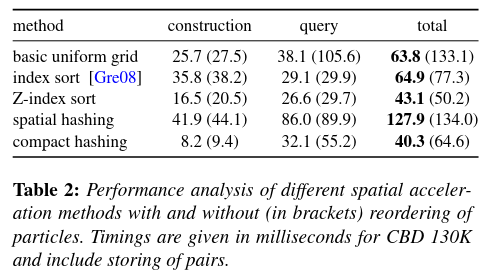
\includegraphics[width=.7\textwidth]{paper-results}
\end{figure}

\end{minipage}
}
\end{frame}

\end{document}
